% this file is called up by thesis.tex
% content in this file will be fed into the main document

\chapter{Research Methodology} % top level followed by section, subsection


% ----------------------- paths to graphics ------------------------

% change according to folder and file names
\ifpdf
    \graphicspath{{4_ResearchMethodology/figures/PNG/}{4_ResearchMethodology/figures/PDF/}{4_ResearchMethodology/figures/}}
\else
    \graphicspath{{4_ResearchMethodology/figures/EPS/}{4_ResearchMethodology/figures/}}
\fi


% ----------------------- contents from here ------------------------

The methodology used to perform stain transfer from H\&E whole slide image patches to the IHC patches leverages a pre-trained Stable Diffusion model with a ControlNet implementation integrated which will be responsible for directed stain transfer. The chapter is organised into distinct phases which are dataset preparation, ControlNet integration, model training and evaluation.

\section{Dataset Preparation}

As mentioned in section 2.2.1.3, this thesis uses the BCI dataset presented by \parencite{Liu2022BCI:Pix2pix}. It is already a fairly well processed and aligned dataset which shall be explored in the subsections below.

\subsection{Dataset Features}

It contains 4,870 H\&E-IHC image pairs of resolution 1024 X 1024 that were cut from the whole slide images of 51 patients. The pairs are distributed across the four IHC HER2 scoring categories which are detailed in Table \ref{tab:HER2 IHC Scoring Guidelines}. The data distribution across these classes of scores is not even, with a disproportionately low number of data points for HER2 score of 0 having only 3 cases available to extract image patches from (Figure \ref{fig:BCI-data-dist}). This data imbalance is an issue and a couple of  potential solutions would be to either augment the classes with cropped, rotated or flipped copies of the images. Another potential solution could be to train the model initially and then generate additional synthetic IHC patches. This could however result in overfitting or adding unseen biases. For the purposes of the thesis, no augmentation was done and the data class distribution was preserved as is.
\begin{figure}[h]
    \centering
    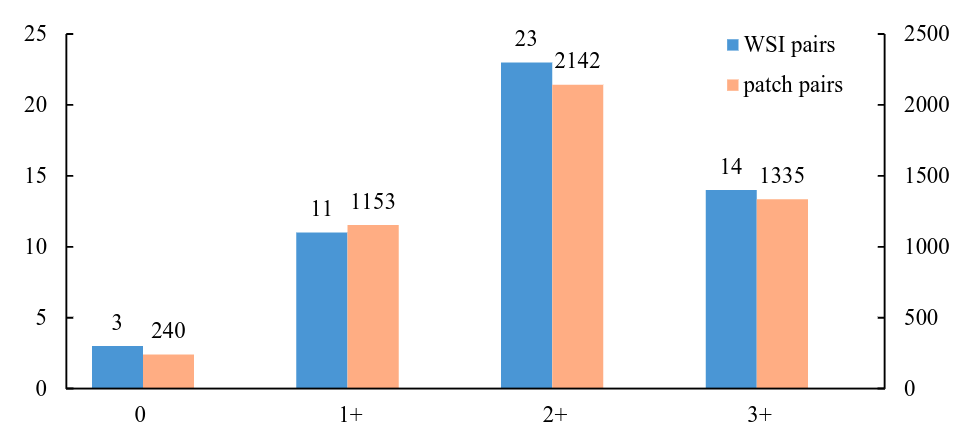
\includegraphics[width=1\linewidth]{4_ResearchMethodology/figures/dataDistribution.png}
    \caption[BCI data distribution]{BCI dataset distribution across the four IHC score classes i.e., 0, 1+, 2+, 3+ \parencite[Figure 8, p. 5]{Liu2022BCI:Pix2pix}}
    \label{fig:BCI-data-dist}
\end{figure}

In terms of the image pairs themselves, they were already structurally aligned by \parencite{Liu2022BCI:Pix2pix} such that they achieve maximum possible overlap. This is achieved by methods of projection transformation and elastix registration \parencite{Klein2010Elastix:Registration}  with the former resulting in a rough overlap between the two image types and subsequently the latter performing a "regional fine-grained non-rigid registration" \parencite[p. 5]{Liu2022BCI:Pix2pix}. 

Though this dataset is very good in terms of pairing and general structural alignment, it is not free of a common issue faced by most such histopathology image datasets which is having a uniform stain colour profile. This is unavoidable in practice as it depends on many factors such as equipment, lighting, etc. Again, in this study, no intentional stain normalisation technique was used. Stress testing the capabilities of Stable Diffusion and allowing for all these variations to see how it would handle it was also a point of interest given its reputation for "artistic sensibilities".

\subsection{Data Preprocessing}

The processing that was done on the data is straightforward. It consisted of applying transforms to it for compatibility with the input channels of the Stable Diffusion model. The transformations made were:

\begin{itemize}
    \item resizing the image from 1024 X 1024 to 512 X 512.
    \item normalising the source H\&E image to [0, 1]
    \item normalising the target IHC image to [-1, 1]
\end{itemize}

The source image is normalised to [0, 1] to ensure stability in training and is the general best practice for faster convergence while the target image is normalised to [-1, 1] to ensure good compatibility with activation functions such as tanh and ReLU  \parencite{Goodfellow2016DeepLearning}.

\subsection{Data split}

The BCI data was already split into train and test classes with there being 3,896 and 977 pairs respectively by \parencite{Liu2022BCI:Pix2pix}. From the 977 test pairs, 40 pairs were moved to a separate validation pair to be used only in the future in the event of final pre-production testing. This provides a split ratio of approximately 80/20. The images are split into two folders namely, ''HE" and "IHC" and there are the three train, test and validation folders inside each that all contain the afore-mentioned splits of images. The file names of the images contain labelling data such as if it is a training image and its IHC score.

In the code implementation, a class called "HE\_IHC\_Dataset" that inherits the PyTorch Dataset class was written and it provides the core dataset access functionality from the file system. It returns a dictionary containing the H\&E image, IHC image, corresponding IHC score as the text prompt and the file name which correspond to the keys, "hint", "jpg", "txt" and "imgName" as seen in code snippet Figure \ref{fig:he-ihc-dataset-class}.  
\begin{figure}[ht]
    \centering
    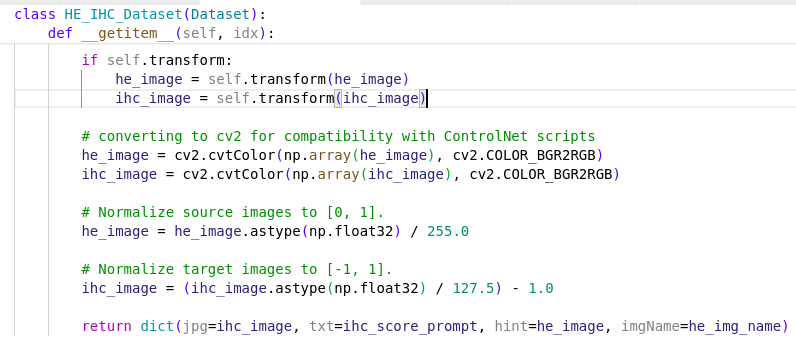
\includegraphics[width=1\linewidth]{4_ResearchMethodology/figures/he_ihc_dataset_class_return_snippet.png}
    \caption[Custom dataset processing class]{Code snippet of custom dataset processing class}
    \label{fig:he-ihc-dataset-class}
\end{figure}

\section{ControlNet Integration}

The fine-tuning code implementation using ControlNet was performed by forking the official ControlNet GitHub repository of \parencite{Zhang2023AddingModels} and creating custom training and testing scripts that incorporate the BCI dataset using the tested and robust ControlNet framework.

\subsection{System Setup}

The experiments were performed on an A100 Nvidia 80GB server GPU. A training loop occupied approximately 30GB of VRAM on the GPU and took approximately 13 hours for 50 training epochs. The pre-trained model of Stable Diffusion used was version 2.1 <TODO: Link to appendix>.

\subsection{Prerequisite}

Before starting the training process, there is a prerequisite to be performed which entails copying the weights of the pre-trained SD model to the trainable copy of ControlNet. This functionality is provided by the framework and only requires the running of  a single python script called. "tool_add_control.py" <TODO: Link to appendix> within the same repository. This script takes two input arguments which are the paths to the downloaded pre-trained SD model in the form of a .ckpt file and the destination path where the trainable copy is to be saved which is also in .ckpt format. This command will look like in the snippet, Figure \ref{fig:copy-sd-control}.
\begin{figure}[h]
    \centering
    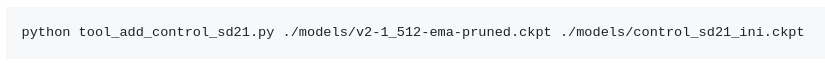
\includegraphics[width=1\linewidth]{4_ResearchMethodology/figures/ckpt_copy.png}
    \caption[Prerequisite command to copy weights]{Prerequisite command to create a duplicate "Control" network from the trained SD model \parencite[GitHub: ControlNet/docs/train.md]{Zhang2023AddingModels}}
    \label{fig:copy-sd-control}
\end{figure}

\subsection{Training}

There were two variations of training conducted. The first had all the Stable Diffusion model's layers locked while the other allowed for the lower decoder blocks' weights to also be re-trained. The Figure \ref{fig:controlnet-sd-locked} 
shows the architecture of a ControlNet's trainable U-Net copy providing additional control information to the locked SD layers at each block. 
\begin{figure}[ht]
    \centering
    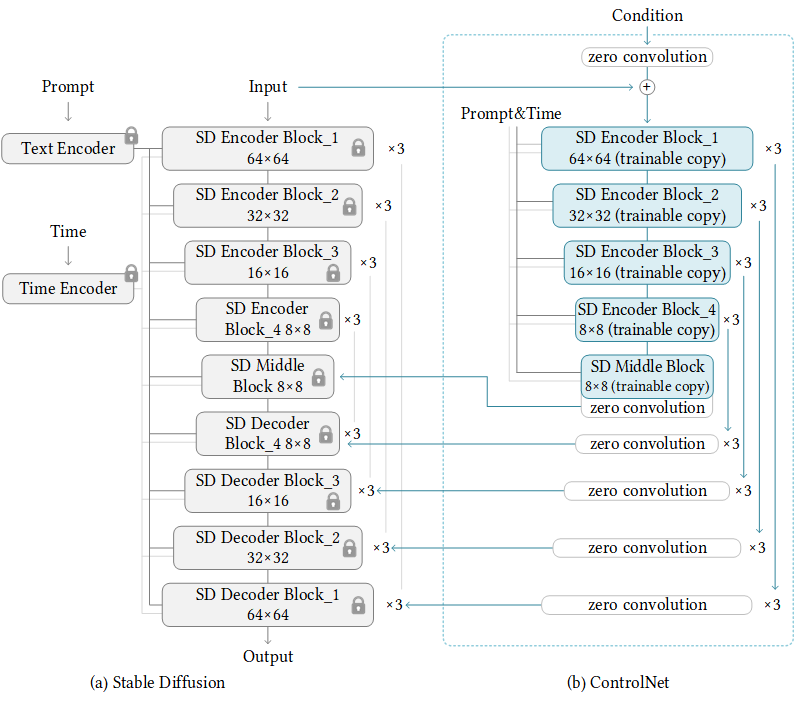
\includegraphics[width=1\linewidth]{4_ResearchMethodology/figures/training_sd_locked.png}
    \caption[ControlNet architecture]{ControlNet implementation with all SD layers locked \parencite[Figure 3, p. 4 ]{Zhang2023AddingModels}}
    \label{fig:controlnet-sd-locked}
\end{figure}
The changes to the hyper-parameters for each variation is tabulated in Table \ref{tab:training-variation} of which there are only two. The second parameter is self-explainable. For the learning rate, going with a slower rate of learning when allowing the weights on the original SD model layers to be trained is recommended because the model will then potentially get downgraded when it learns only from a new specific source of data.

\begin{table}[H]
\begin{center}
\begin{tabular}{|>{\raggedright\arraybackslash}p{0.3\linewidth}|>{\raggedright\arraybackslash}p{0.35\linewidth}|>{\raggedright\arraybackslash}p{0.35\linewidth}|}
\hline 
\textbf{}& \textbf{SD Locked}& \textbf{SD Unlocked}\\ \hline 
Hyper-parameters& learning rate = $1e^{-5}$, sd\_locked = True& learning rate = $2e^{-6}$, sd\_locked = False\\ \hline
\end{tabular}
\caption[Hyper-parameter differences between ControlNet training variations]{Hyper-parameter differences between ControlNet training variations}\label{tab:training-variation}
\end{center}
\end{table}
Other than these, the constant hyper-parameters used are a batch size of 4, the AdamW optimiser for its better control over regularisation \parencite{Loshchilov2017DecoupledRegularization}, a standard Mean Square Error (MSE) loss function and number of epochs each of 50. 

\section{Evaluation}

Comparing and evaluating the results for this project is not a straightforward task. The task of comparing an image to an attempted imitation of it is not a process that any algorithm can decipher easily. The results of this type where structural variations can be acceptable if the overall pattern is very similar to the original can have merits and can be enough for providing a highly accurate IHC score that can inform pathologists faster than the manual scoring method. 

Nonetheless, for this thesis, two main categories of evaluation were carried out; quantitative and qualitative. The quantitative method consists of using the Peak Signal to Noise Ratio (PSNR) and Structural Similarity (SSIM) evaluation metrics. PSNR performs a rigid pixel-to-pixel comparison which does not really paint the full picture while the SSIM method takes into account the differences in the image brightness, contrast and structure. While still not a very good benchmark to fully analyse a pair of results, it is certainly fair than PSNR.

For qualitative testing, a random sample size of 20 generated IHC images were chosen via a python script <TODO: add appendix link to code> to avoid any selection bias and were independently evaluated by an expert Pathologist. The pathologist's score was compared against the actual score the target image was categorised into and a simple sum and average of successes was calculated to determine the accuracy of the test. The evaluation and results are discussed in the chapter 4.

% ---------------------------------------------------------------------------
% ----------------------- end of thesis sub-document ------------------------
% ---------------------------------------------------------------------------